\documentclass[a4paper,14pt]{extreport}

% =====Задание кодировки=====
\usepackage[utf8]{inputenc}
\usepackage[english,russian]{babel}

\usepackage{fontspec}
\setmainfont[Ligatures=TeX]{Liberation Serif}
\setsansfont[Ligatures=TeX]{Liberation Sans}
% ===========================



% =====Размеры полей=====
\usepackage[left=3cm, right=1.5cm, vmargin=2cm]{geometry}
% =======================



% =====Полуторный интервал=====
\linespread{1.25}
% =============================



% =====Красная строка=====
\usepackage{indentfirst}
\setlength\parindent{1.25cm}
% ========================



% =====Формат заголовков=====
\usepackage{titlesec}

\titleformat
	{\chapter}
	[block]
	{\filcenter\bfseries}
	{\thechapter}
	{1ex}{}
\titlespacing{\chapter}{0pt}{*1}{*1}

\titleformat
	{\section}
	[block]
	{\hspace{\parindent}\bfseries}
	{\thesection}
	{1ex}{}
\titlespacing{\section}{0pt}{*1}{*1}

\titleformat
	{\subsection}
	[block]
	{\hspace{\parindent}\bfseries}
	{\thesubsection}
	{1ex}{}
\titlespacing{\subsection}{0pt}{*1}{*1}

\titleformat
	{\subsubsection}
	[runin]
	{\bfseries}
	{\thesubsubsection}
	{1ex}{}[. ]
\titlespacing{\subsubsection}{1.25cm}{*1}{*1}

\titleformat
	{\paragraph}
	[runin]
	{\bfseries}
	{\theparagraph}
	{1ex}{}[. ]
\titlespacing{\paragraph}{1.25cm}{*1}{*1}

\setcounter{secnumdepth}{3}
% ===========================



% =====Содержание=====
\addto{\captionsrussian}{\renewcommand*{\contentsname}{СОДЕРЖАНИЕ}}
\usepackage{titletoc}
\dottedcontents{chapter}[0em]{\bfseries}{1em}{1ex}
\dottedcontents{section}[2em]{}{2em}{1ex}
\dottedcontents{subsection}[5em]{}{3em}{1ex}
\usepackage[hidelinks]{hyperref}
% ====================



% =====Поиск по тексту=====
\usepackage{cmap}
% =========================



% =====Выравнивание текста=====
\usepackage{ragged2e}
\usepackage{microtype}
\justifying
\sloppy
\tolerance=500
\hyphenpenalty=10000
\emergencystretch=3em
% =============================



% =====Списки====
\renewcommand{\labelitemi}{--}
\renewcommand{\labelitemii}{--}

\renewcommand{\labelenumi}{\asbuk{enumi})}
\renewcommand{\labelenumii}{\arabic{enumii})}

\usepackage{enumitem}
\makeatletter
\AddEnumerateCounter{\asbuk}{\@asbuk}{ю)}
\makeatother
\setlist{nosep,wide}
\setlist[2]{labelindent=2\parindent}
% ===============



% =====Поддержка изображений и таблиц=====
\usepackage[tableposition=top,singlelinecheck=false]{caption}
\usepackage{subcaption}
\usepackage{multirow}
\usepackage{graphicx}
\usepackage{float}
\usepackage{tabularx,ragged2e,booktabs}

\DeclareCaptionLabelFormat{gostfigure}{Рисунок #2}
\DeclareCaptionLabelFormat{gosttable}{Таблица #2}
\DeclareCaptionLabelSeparator{gost}{~---~}
\captionsetup{labelsep=gost}
\captionsetup*[figure]{labelformat=gostfigure,justification=centering}
\captionsetup*[table]{labelformat=gosttable}
\renewcommand{\thesubfigure}{\asbuk{subfigure}}
% ===============================



% Запускать pdflatex с --shell-escape
% =====Листинги=====
\usepackage{minted}
% ==================



\begin{document}
	
\thispagestyle{empty}
\begin{center}

МИНИСТЕРСТВО ВЫСШЕГО ОБРАЗОВАНИЯ И НАУКИ РОССИЙСКОЙ ФЕДЕРАЦИИ
ФЕДЕРАЛЬНОЕ ГОСУДАРСТВЕННОЕ БЮДЖЕТНОЕ
ОБРАЗОВАТЕЛЬНОЕ УЧРЕЖДЕНИЕ
ВЫСШЕГО ОБРАЗОВАНИЯ

«НОВОСИБИРСКИЙ ГОСУДАРСТВЕННЫЙ ТЕХНИЧЕСКИЙ УНИВЕРСИТЕТ»

\noindent\rule{\textwidth}{0.4pt}

Кафедра вычислительной техники

\begin{figure}[H]
	\centering
	
\includegraphics{title/logo.jpeg}
\end{figure}

Лабораторная работа №3

По дисциплине: «Программное обеспечение информационных систем»

По теме: «Приложение ASP.NET Core для работы с базой данных PostgreSQL»

\end{center}

\noindent\begin{tabular}{p{0.5\textwidth}p{0.5\textwidth}}
	Выполнили: & Проверил: \\
	Студенты гр. <<АВТ-818>>, <<АВТФ>> & << должность >>\\
	<<Жигулин И. О.>> & <<Бычков М. И.>> \\
	<<Сороковикова Е. В.>> & \\
	<<\rule{1.5em}{0.4pt}>> \rule{5em}{0.4pt} 20\rule{1.5em}{0.4pt}г. & <<\rule{1.5em}{0.4pt}>> \rule{5em}{0.4pt} 20\rule{1.5em}{0.4pt}г.\\
	\rule{7.5em}{0.4pt} & \rule{7.5em}{0.4pt} \\
	\hspace{1.5em}(подпись) & \hspace{1.5em}(подпись)
\end{tabular}


\begin{center}

\vspace{2.3cm}

Новосибирск

2021
\end{center}


\tableofcontents

\chapter{Введение}

\section{Цель работы}

\begin{itemize}
	\item получить базовые навыки работы в среде R;
	\item изучить средства R для проведения первичного разведочного анализа данных (методы визуализации, описательной статистики, корреляционного анализа данных) на примере решения конкретной задачи ИАД (интеллектуального анализа данных).
\end{itemize}


\section{Задание для варианта №5}
Изучаются показатели работы программистов крупной организации. Рассматриваются следующие показатели (признаки) для каждого программиста:

\begin{itemize}
	\item пол (1-м, 2-ж);
	\item возраст;
	\item стаж работы;
	\item процент разработок, выполненных в срок в рамках бюджета с требуемым функционалом (за год);
	\item количество ошибок, выявленных пользователем (за год);
	\item стаж работы по специальности в данной организации;
	\item степень удовлетворенности заказчика;
	\item качество документирования (1 – низкое, 2 – среднее, 3 – выше среднего, 4- высокое).
\end{itemize}

Необходимо провести предварительный разведочный анализ данных с целью описания характера распределения данных, выявления структуры взаимосвязей между показателями.

Программисты разбиты на две группы в зависимости от стажа работы:

\begin{itemize}
	\item 1 группа - стаж менее 4
	\item 2 группа - стаж более 4
\end{itemize}

\chapter{Организация выполнения пакетной обработки}

\section{Перечень и основные характеристики программного обеспечения}

Несмотря на то, что средства MPI сами по себе позволяют осуществлять запуск параллельных задач, обычно для этих целей используются различные менеджеры ресурсов.

Можно назвать следующее программное обеспечение для управления кластером:

\begin{itemize}
	\item Torque,
	\item Maui,
	\item Corosync.
\end{itemize}

\paragraph{Torque}
Менеджер распределённых ресурсов для вычислительных кластеров из машин под управлением Linux и других Unix-подобных операционных систем, одна из современных версий Portable Batch System (PBS). Распространяется под свободной лицензией OpenPBS Software License. TORQUE разрабатывается и поддерживается сообществом на базе проекта OpenPBS. Для менеджера существует более 1200 патчей и расширений, написанных крупнейшими организациями и лабораториями, среди которых US DOE, USC, PNLL и др., это позволяет достичь высокой степени масштабируемости и отказоустойчивости менеджера как системы.

\paragraph{Maui}
Планировщик заданий в параллельных и распределенных вычислительных системах (кластерах). Как правило, используется совместно с менеджером распределенных ресурсов TORQUE.
Maui позволяет выбирать различные политики планирования, поддерживает динамическое изменение приоритетов, исключения. Все это улучшает управляемость и эффективность машин, начиная от простых кластеров до суперкомпьютеров.

\paragraph{Corosync}
Проект с открытым исходным кодом, реализующий систему группового общения для отказоустойчивых кластеров. Является развитием проекта OpenAIS и опубликован в соответствии с модифицированной лицензией BSD. Программное обеспечение создано как исполняемые бинарные файлы, использующие клиент-серверную модель взаимодействия между библиотеками и сервисными инструментами. Модули, называемые сервисными инструментами, загружаются в Corosync и используют сервисы, предоставляемые внутренним API Corosync.

В ходе выполнения лабораторной работы будет произведено развертывание системы Torque.

\section{Развертывание системы Torque}
Torque главным образом используется на многопроцессорных вычислительных установках. Объединение ресурсов в них обычно уменьшает необходимость в постоянном управлении ресурсами для пользователей. Настроенная однажды правильно вычислительная установка абстрагируется от многих деталей, связанных с запуском и управлением заданиями. Пользователю обычно надо установить в параметрах лишь минимальные требования к задаче, и ему нет необходимости знать даже имена вычислительных узлов, на которых задача выполняется.


\section{Запуск параллельных программ и скриптов}


\section{Результат тестирования}


\chapter{ЗАКЛЮЧЕНИЕ}

\section{Демонстрация работы}

\begin{figure}[H]
	\centering
	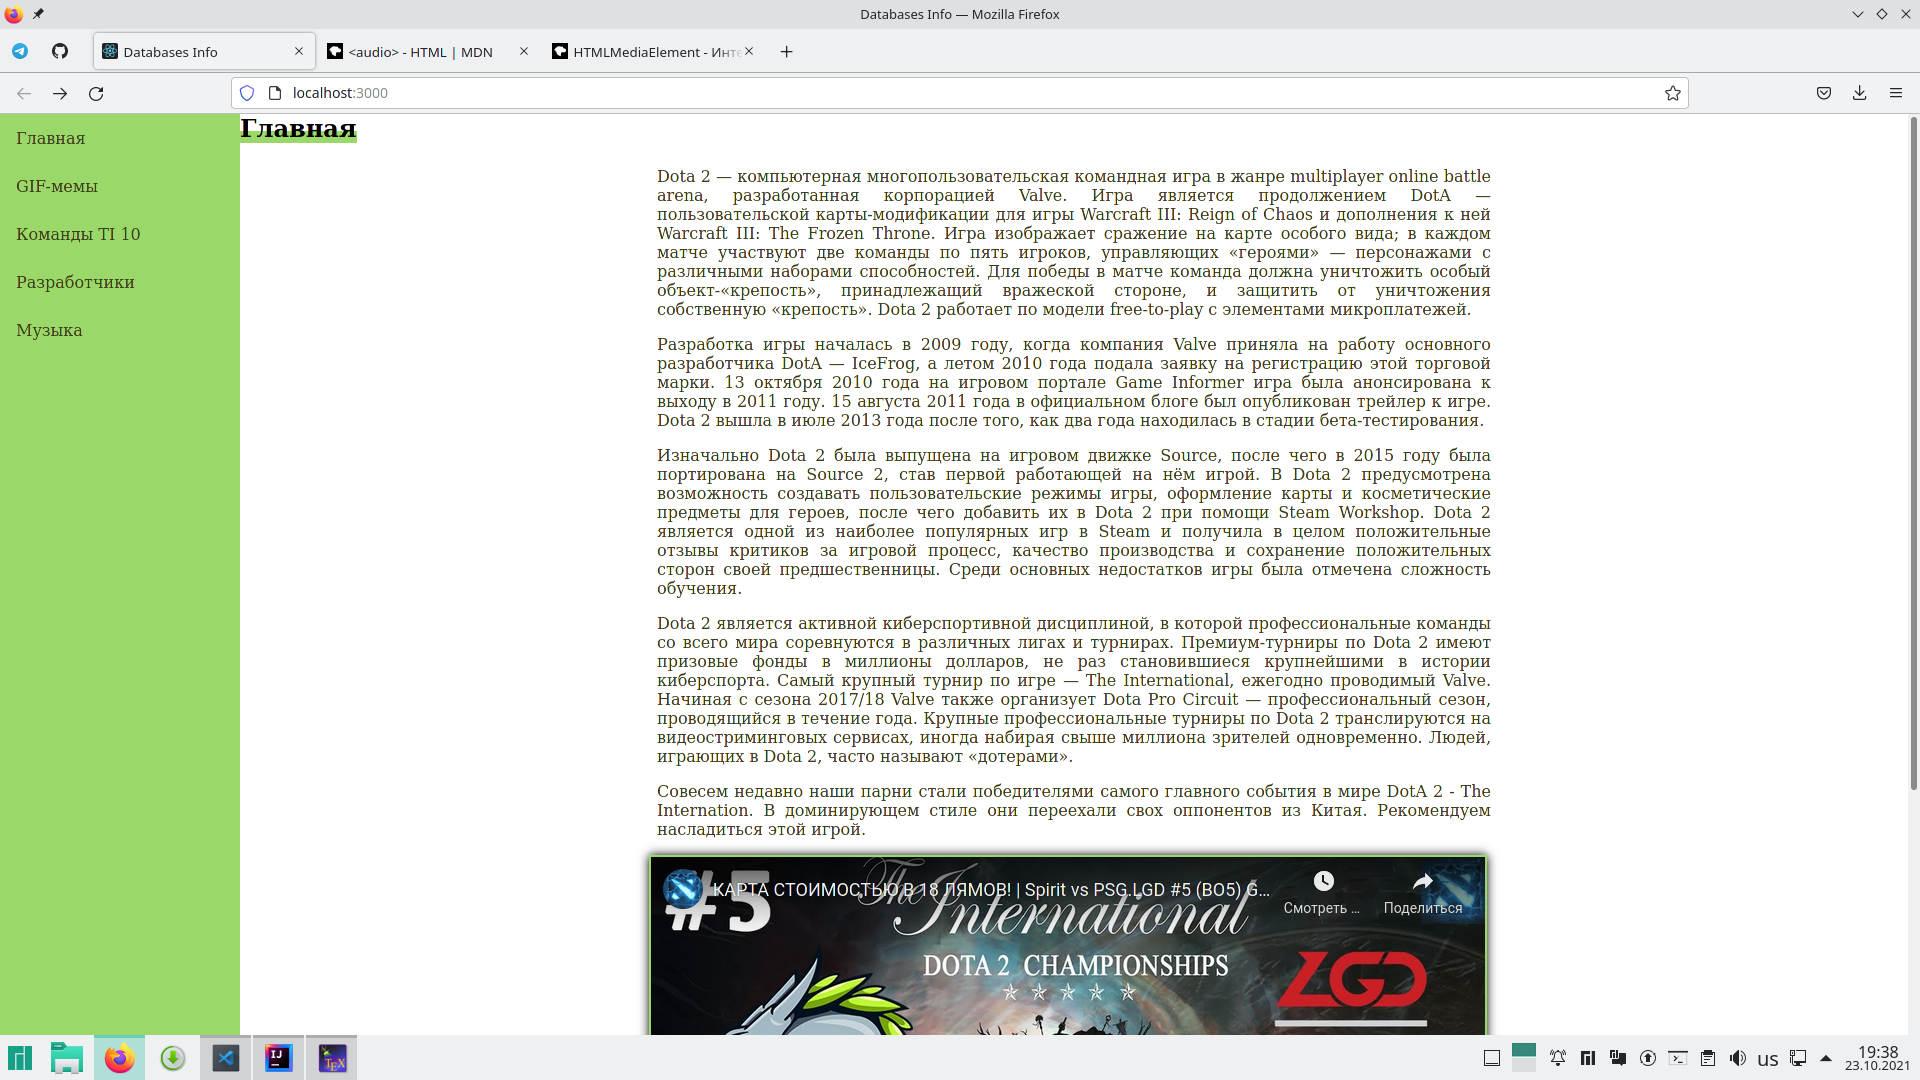
\includegraphics[width=0.7\textwidth]{01}
	\caption{Сохраненная база данных}
\end{figure}

\begin{figure}[H]
	\centering
	
\includegraphics[width=0.7\textwidth]{02}
	\caption{Файл JSON базы данных}
\end{figure}

\begin{figure}[H]
	\centering
	
\includegraphics[width=0.7\textwidth]{03}
	\caption{База данных после очистки}
\end{figure}

\begin{figure}[H]
	\centering
	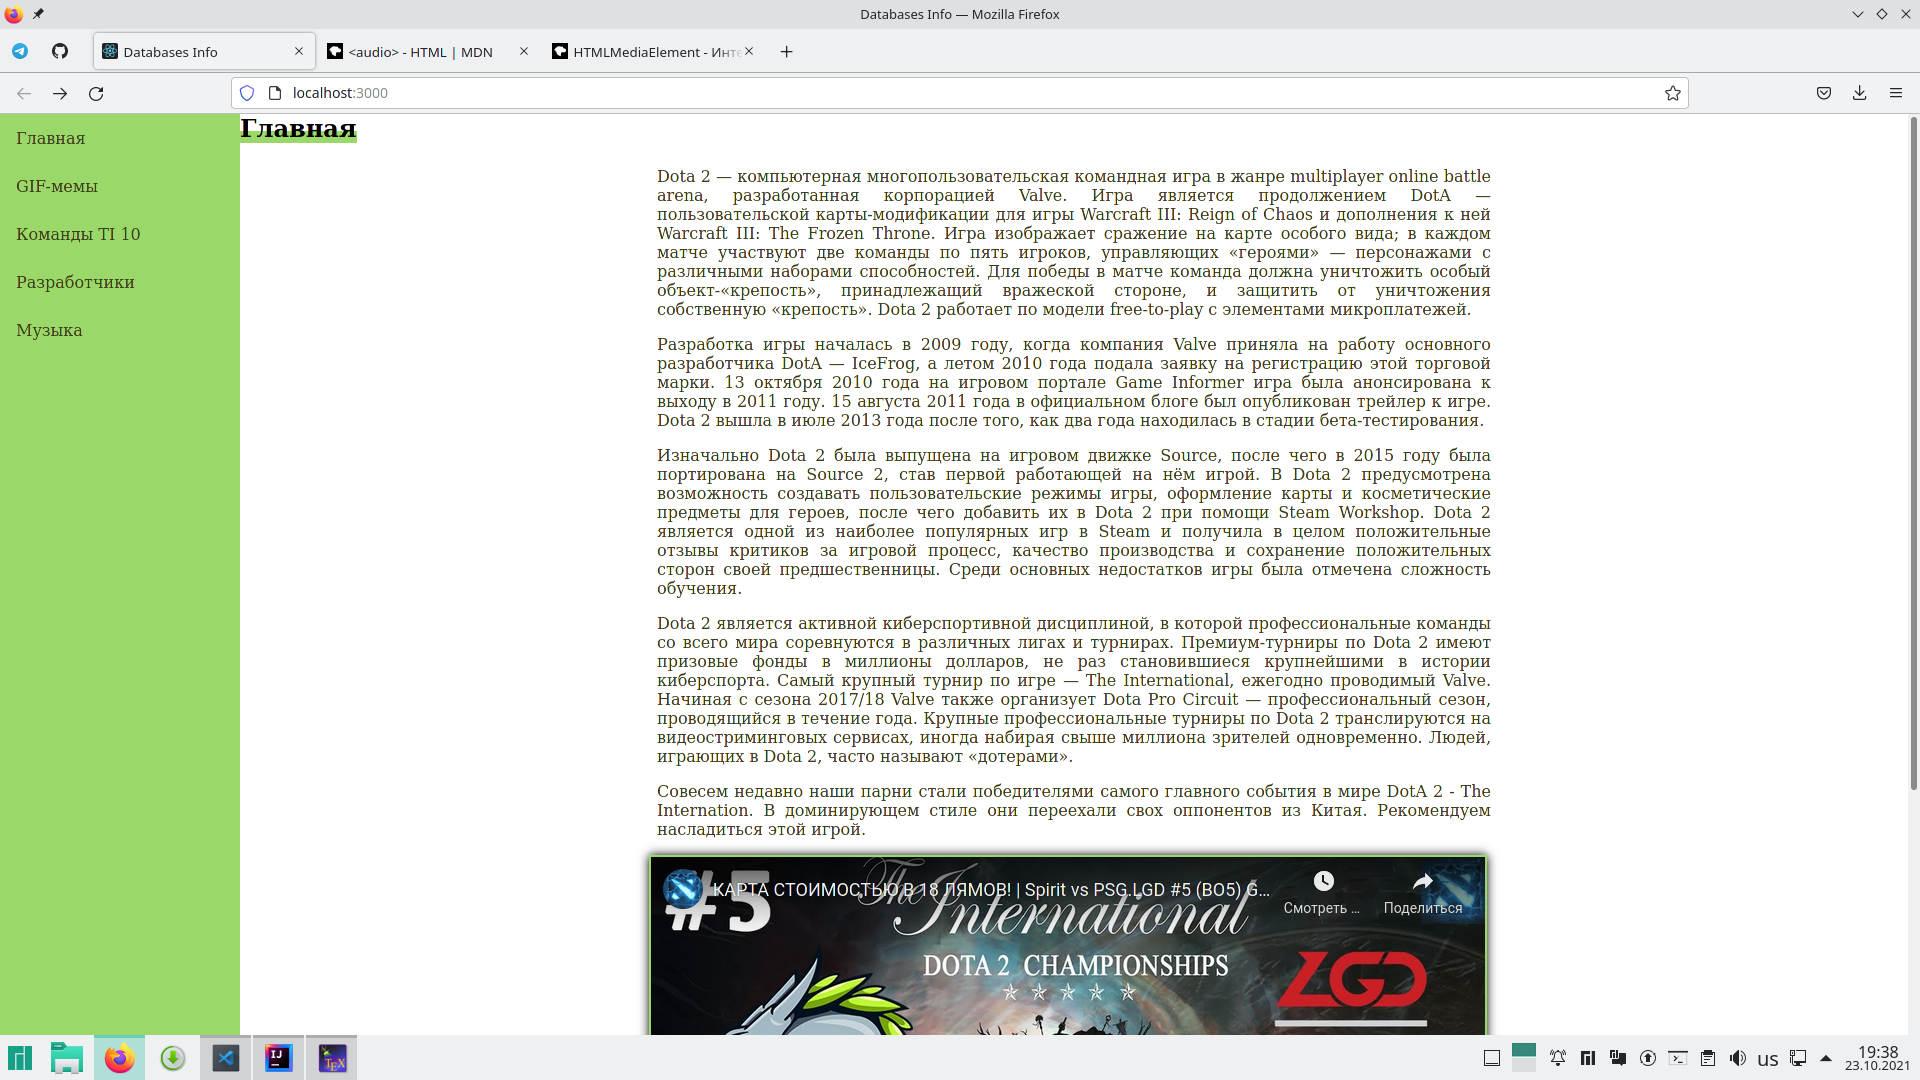
\includegraphics[width=0.7\textwidth]{01}
	\caption{База данных после восстановления}
\end{figure}

\section{Вывод}
В ходе выполнения лабораторной работы были реализованы:
\begin{enumerate}
	\item Запись данных из БД в файл формата JSON.
	\item Очистка данных из БД.
	\item Загрузка данных в БД из файла в формате JSON.
\end{enumerate}


\end{document}